\documentclass{article}\usepackage[]{graphicx}\usepackage[]{color}
%% maxwidth is the original width if it is less than linewidth
%% otherwise use linewidth (to make sure the graphics do not exceed the margin)
\makeatletter
\def\maxwidth{ %
  \ifdim\Gin@nat@width>\linewidth
    \linewidth
  \else
    \Gin@nat@width
  \fi
}
\makeatother

\definecolor{fgcolor}{rgb}{0.345, 0.345, 0.345}
\newcommand{\hlnum}[1]{\textcolor[rgb]{0.686,0.059,0.569}{#1}}%
\newcommand{\hlstr}[1]{\textcolor[rgb]{0.192,0.494,0.8}{#1}}%
\newcommand{\hlcom}[1]{\textcolor[rgb]{0.678,0.584,0.686}{\textit{#1}}}%
\newcommand{\hlopt}[1]{\textcolor[rgb]{0,0,0}{#1}}%
\newcommand{\hlstd}[1]{\textcolor[rgb]{0.345,0.345,0.345}{#1}}%
\newcommand{\hlkwa}[1]{\textcolor[rgb]{0.161,0.373,0.58}{\textbf{#1}}}%
\newcommand{\hlkwb}[1]{\textcolor[rgb]{0.69,0.353,0.396}{#1}}%
\newcommand{\hlkwc}[1]{\textcolor[rgb]{0.333,0.667,0.333}{#1}}%
\newcommand{\hlkwd}[1]{\textcolor[rgb]{0.737,0.353,0.396}{\textbf{#1}}}%

\usepackage{framed}
\makeatletter
\newenvironment{kframe}{%
 \def\at@end@of@kframe{}%
 \ifinner\ifhmode%
  \def\at@end@of@kframe{\end{minipage}}%
  \begin{minipage}{\columnwidth}%
 \fi\fi%
 \def\FrameCommand##1{\hskip\@totalleftmargin \hskip-\fboxsep
 \colorbox{shadecolor}{##1}\hskip-\fboxsep
     % There is no \\@totalrightmargin, so:
     \hskip-\linewidth \hskip-\@totalleftmargin \hskip\columnwidth}%
 \MakeFramed {\advance\hsize-\width
   \@totalleftmargin\z@ \linewidth\hsize
   \@setminipage}}%
 {\par\unskip\endMakeFramed%
 \at@end@of@kframe}
\makeatother

\definecolor{shadecolor}{rgb}{.97, .97, .97}
\definecolor{messagecolor}{rgb}{0, 0, 0}
\definecolor{warningcolor}{rgb}{1, 0, 1}
\definecolor{errorcolor}{rgb}{1, 0, 0}
\newenvironment{knitrout}{}{} % an empty environment to be redefined in TeX

\usepackage{alltt}
\usepackage{fullpage, amssymb, url, natbib}
\usepackage[colorlinks = true, linkcolor = blue, urlcolor  = blue, citecolor = blue,
anchorcolor = blue]{hyperref}
\IfFileExists{upquote.sty}{\usepackage{upquote}}{}
\begin{document}

\begin{knitrout}
\definecolor{shadecolor}{rgb}{0.969, 0.969, 0.969}\color{fgcolor}\begin{kframe}


{\ttfamily\noindent\color{warningcolor}{\#\# Warning: package 'car' was built under R version 3.1.3}}

{\ttfamily\noindent\color{warningcolor}{\#\# Warning: package 'lattice' was built under R version 3.1.3}}

{\ttfamily\noindent\color{warningcolor}{\#\# Warning: package 'ggplot2' was built under R version 3.1.3}}\end{kframe}
\end{knitrout}


\noindent Albert Y. Kim\\
Adriana Escobedo-Land\\
Reed College\\
OkCupid Profile Data for Introductory Statistics and Data Science Courses\\

\noindent \textbf{Keywords}: OkCupid, online dating, data science, big data.

\begin{abstract}

WRITE THIS

\end{abstract}










%------------------------------------------------------------------------------
%
\section{Introduction}\label{intro}
%
%------------------------------------------------------------------------------
In light of the field of data science gaining more prominence in academia, industry, and government, many statisticians are arguing that statistics needs to stake a bigger claim in data science in order to avoid marginalization by other disciplines such as computer science and computer engineering~\cite{YU:2014,DAVIDSON:2014}.  While precise definition of the difference between statistics and data science and its implications for statistics education can be debated~\cite{WICKHAM:2014}, one consensus among many in statistics education circles is that at the very least statistics needs to incorporate a heavier computing component and the use of technology for both developing conceptual understanding and analyzing data~\cite{GAISE:05, NOLAN:LANG:2010}.  Relatedly, in the hopes of making introductory undergraduate statistics courses more relevant, many statistics educators are placing a higher emphasis on the use of real data in the classroom, a practice the American Statistical Association's Guidelines for Assessment and Instruction in Statistics Education (GAISE) project's reports strongly encourages~\cite{GAISE:05}.  Of particular importance in the success of such ambitions are the data sets considered, as they provide the context of the analyses and thus will ultimately drive student interest~\cite{GOULD:2010}.

It is in light of these discussions that we present this paper centering on data from the online dating website OkCupid, specifically a snapshot of San Francisco California users taken on June 2012.  We describe the dataset and present a series of example analyses along with corresponding pedagogical discussions.  The example analyses presented in this paper were used in a variety of settings at Reed College: a 90 minute introductory tutorial on R, an introductory probability and statistics class, and a follow-up two-hundred level data science class titled ``Case Studies in Statistical Analysis.''  Statistical and data science concepts covered include basic data visualizations, exploratory data analyses, multivariate relationships, text analysis, and logistic regression for prediction.  All examples are presented using the R statistical software program and using the \verb#mosaic#, \verb#dplyr#, \verb#stringr#, and \verb#ggplot2# packages~\cite{mosaic, dplyr, stringr, ggplot2}.








%------------------------------------------------------------------------------
%
\section{Data}
%
%------------------------------------------------------------------------------
The data consists of the public profiles of 59,946 OkCupid users who were living within 25 miles of San Francisco, had active profiles on June 26, 2012, were online in the previous year and had at least one picture in their profile.  Using a Python script, data was scraped from users' public profiles on June 30, 2012; any non-publicly facing information such as messaging and login behavior was not accessible.

Variables include typical user information (such as sex, sexual orientation, age, and ethnicity) and lifestyle variables (such as diet, drinking habits, smoking habits).  Furthermore, text strings of the responses to the 10 essay questions posed to all OkCupid users are included as well, such as ``My Self Summary'', ``The first thing people usually notice about me...'', and ``On a typical Friday night I am...''  For a complete list of variables and more details, see the accompanying codebook \verb#okcupid_codebook.txt#.

\begin{knitrout}
\definecolor{shadecolor}{rgb}{0.969, 0.969, 0.969}\color{fgcolor}\begin{kframe}
\begin{alltt}
\hlstd{profiles} \hlkwb{<-} \hlkwd{read.csv}\hlstd{(}\hlkwc{file}\hlstd{=}\hlstr{"profiles.csv"}\hlstd{,} \hlkwc{header}\hlstd{=}\hlnum{TRUE}\hlstd{,} \hlkwc{stringsAsFactors}\hlstd{=}\hlnum{FALSE}\hlstd{)}
\hlstd{n} \hlkwb{<-} \hlkwd{nrow}\hlstd{(profiles)}
\end{alltt}
\end{kframe}
\end{knitrout}

Analysis of similar data has received much press of late, including Amy Webb's TED talk ``How I Hacked Online Dating''~\cite{TED} and Wired magazine's ``How a Math Genius Hacked OkCupid to Find True Love''~\cite{Wired}.  OkCupid co-founder Christian Rudder pens periodical analysis of their data via the OkTrends blog~\cite{OkTrends} and has recently published a book ``Dataclysm: Who We Are When We Think No One's Looking'' describing similar data driven insights~\cite{dataclysm}.  Such publicity surrounding data-driven online dating and the salience of dating matters among students makes this dataset one with much potential to be of interest to students, hence facilitating the instruction of statistical and data science concepts.

Before we continue we note that even though this data consists of publicly facing material, one should proceed with caution before scraping then using data in fashion similar to ours, as the Computer Fraud and Abuse Act (CFAA) makes it a federal crime to access a computer without authorization from the owner~\cite{pando}.  In our case, permission was given by the owners of the data (See Section \ref{ack}).










%------------------------------------------------------------------------------
%
\section{Example Analyses}\label{analyses}
%
%------------------------------------------------------------------------------
The example analyses we present address the following questions:

\begin{enumerate}
\item How do the heights of male and female OkCupid users compare?
\item What does the San Francisco online dating landscape look like?  Or more specifically, what is the relationship between users' sex and sexual orientation?
\item Are there differences between the sexes in what words are used in the responses to the 10 essay questions?
\item Can we predict a users' sex using profile information?
\end{enumerate}




%---------------------------------------------------------------
\subsection{Male and Female Heights}\label{section_height}
%---------------------------------------------------------------
\subsubsection{Exercise}
We compare the distribution of OkCupid user's heights between men and women.  Height is one of 3 numerical variables in this dataset (the others being height and income).  This provides us an opportunity to investigate numerical summaries using the \verb#favstats()# command from the \verb#mosaic# package:

\begin{center}
\begin{knitrout}
\definecolor{shadecolor}{rgb}{0.969, 0.969, 0.969}\color{fgcolor}\begin{kframe}
\begin{alltt}
\hlkwd{favstats}\hlstd{(height,} \hlkwc{data}\hlstd{=profiles)}
\end{alltt}
\begin{verbatim}
##  min Q1 median Q3 max mean sd     n missing
##    1 66     68 71  95   68  4 59943       3
\end{verbatim}
\end{kframe}
\end{knitrout}
\end{center}

We observe that some of the heights are nonsensical, including heights of 1 inch and 95 inches (equaling 7'11'').  We deem heights between 55 and 80 inches to be reasonable, and while there is potential bias in discarding users with non-reasonable heights, since out of the 59946 users there are only 117 who would be discarded, we proceed anyways.  We keep only those users with heights between 55 and 80 inches either using the \verb#subset()# command or using the \verb#filter()# command from \verb#dplyr# package. Note that the following commands are equivalent:

\begin{knitrout}
\definecolor{shadecolor}{rgb}{0.969, 0.969, 0.969}\color{fgcolor}\begin{kframe}
\begin{alltt}
\hlstd{profiles.subset} \hlkwb{<-} \hlkwd{subset}\hlstd{(profiles, height}\hlopt{>=}\hlnum{55} \hlopt{&} \hlstd{height} \hlopt{<=}\hlnum{80}\hlstd{)}
\hlstd{profiles.subset} \hlkwb{<-} \hlkwd{filter}\hlstd{(profiles, height}\hlopt{>=}\hlnum{55} \hlopt{&} \hlstd{height} \hlopt{<=}\hlnum{80}\hlstd{)}
\end{alltt}
\end{kframe}
\end{knitrout}

We compare the distributions of male and female heights using histograms.  While we could plot two separate histograms without regard to the scale of the x-axis, in Figure \ref{fig:heights_by_sex} we instead

\begin{enumerate}
\item Plot them with bin widths matching the granularity of the observations (inches)
\item Plot them simultaneously in a panel consisting of two rows and one column of plots using the command \verb#par(mfrow=c(2,1))#
\item Plot them with the same scale on the x-axis (by matching the histograms' \verb#breaks=55:80#) and the y-axis (by selecting the density and not frequency using \verb#prob=TRUE#) to facilitate comparisons between the two distributions
\end{enumerate}


\begin{knitrout}
\definecolor{shadecolor}{rgb}{0.969, 0.969, 0.969}\color{fgcolor}\begin{kframe}
\begin{alltt}
\hlstd{profiles.male} \hlkwb{<-} \hlkwd{filter}\hlstd{(profiles.subset, sex}\hlopt{==}\hlstr{'m'}\hlstd{)}
\hlstd{profiles.female} \hlkwb{<-} \hlkwd{filter}\hlstd{(profiles.subset, sex}\hlopt{==}\hlstr{'f'}\hlstd{)}
\hlkwd{par}\hlstd{(}\hlkwc{mfrow}\hlstd{=}\hlkwd{c}\hlstd{(}\hlnum{2}\hlstd{,}\hlnum{1}\hlstd{))}
\hlkwd{hist}\hlstd{(profiles.female}\hlopt{$}\hlstd{height,} \hlkwc{breaks}\hlstd{=}\hlnum{55}\hlopt{:}\hlnum{80}\hlstd{,} \hlkwc{main}\hlstd{=}\hlstr{"Females"}\hlstd{,} \hlkwc{prob}\hlstd{=}\hlnum{TRUE}\hlstd{,} \hlkwc{xlab}\hlstd{=}\hlstr{"Height (in.)"}\hlstd{)}
\hlkwd{hist}\hlstd{(profiles.male}\hlopt{$}\hlstd{height,} \hlkwc{breaks}\hlstd{=}\hlnum{55}\hlopt{:}\hlnum{80}\hlstd{,} \hlkwc{main}\hlstd{=}\hlstr{"Males"}\hlstd{,} \hlkwc{prob}\hlstd{=}\hlnum{TRUE}\hlstd{,} \hlkwc{xlab}\hlstd{=}\hlstr{"Height (in.)"}\hlstd{)}
\end{alltt}
\end{kframe}\begin{figure}

{\centering 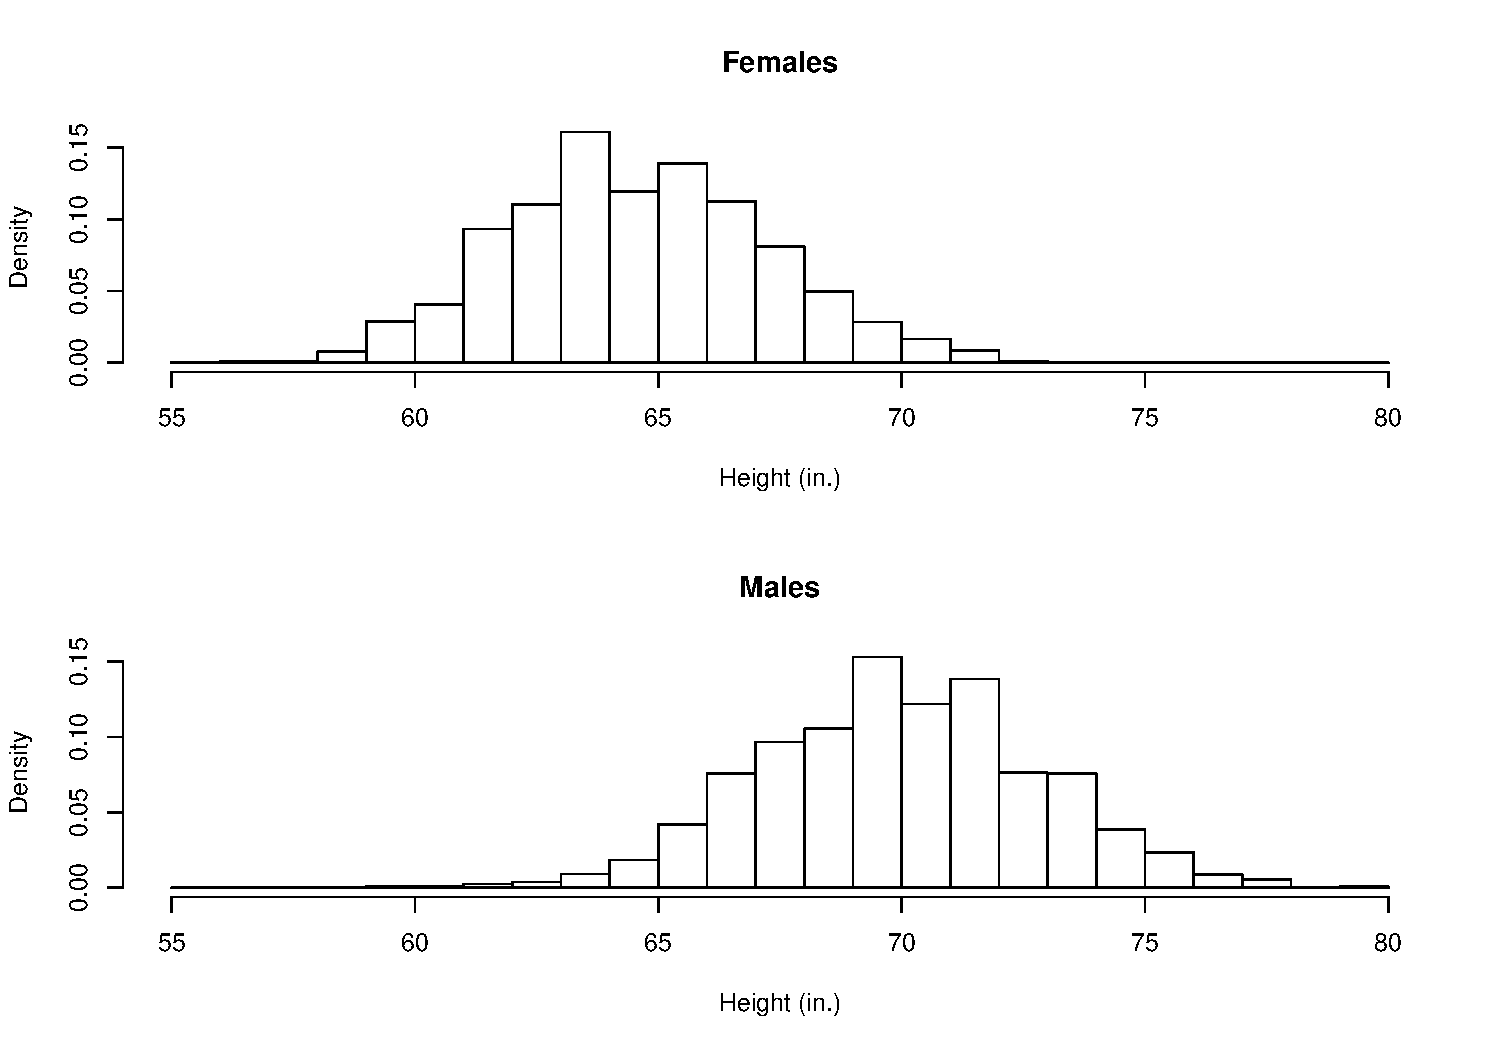
\includegraphics[width=\maxwidth]{figure/heights_by_sex-1} 

}

\caption[Histograms of user heights split by sex]{Histograms of user heights split by sex.}\label{fig:heights_by_sex}
\end{figure}


\end{knitrout}


\subsubsection{Pedagogical Discussion}
This first exercise stresses many important considerations students should keep in mind when working with real data.  Firstly, it emphasizes the importance of performing an exploratory data analysis to identify anomalous observations and confronts students with the question of what to do with them.  For example, while a height of 1 inch is clearly an outlier that needs to be removed, at what point does a height no longer become reasonable and what impact does their removal have on the conclusions?  In our case, since only a small number of observations were removed, the impact would be minimal.

Secondly, this exercise demonstrates the power of data visualizations as simple as histograms to convey insight and hence emphasizes the importance of putting careful thought into their construction.  In our case, while having students plot two histograms simultaneously on the same scale in order to demonstrate that males have on average greater height may seem to be a rather pedantic goal at first, we encouraged students to take a closer look at the histograms and steered their focus towards the unusual peaks at 72 inches (6 feet) for males and 64 inches (5'4'') for females.  Many of the students could explain the phenomena of the peak at 72 inches for men: sociological perceptions of the rounded height of 6 feet.  On the other hand, consensus was not as strong about perceptions of the height of 5'4'' for women.  Instructors can then refer students to the entry on OkCupid's blog OkTrends ``The Biggest Lies in Online Data''\cite{OkTrendsLies} to show they've replicated (on a smaller scale) a previous analysis and then show other analyses conducted by OkCupid.

Further questions that can be pursued from this exercise include ``How can we question if those peaks are significant or due to chance?'', ``Are we only observing men who are just under 6 feet rounding up, or are men just over 6 feet rounding down as well?'', or ``How can we compare the distribution of listed heights on OkCupid to the actual San Francisco population's height distribution?''







%---------------------------------------------------------------
\subsection{Relationship Between Sex and Sexual Orientation}\label{sex_by_sexual_orientation}
%---------------------------------------------------------------
\subsubsection{Exercise}
Since among the most important considerations in assessing a potential mate are their sex and sexual orientation, in this exercise we investigate the relationship between these two variables.  At the time, OkCupid allowed for two possible sex choices (male or female) and three possible sexual orientation (gay, bisexual, or straight)\footnote{OkCupid has since relaxed these categorizations to allow for a broader range of choices for both sex and sexual orientation}.  First, we perform a basic exploratory data analysis on these variables using barcharts in Figure \ref{fig:sex_and_orientation}:

\begin{knitrout}
\definecolor{shadecolor}{rgb}{0.969, 0.969, 0.969}\color{fgcolor}\begin{kframe}
\begin{alltt}
\hlkwd{par}\hlstd{(}\hlkwc{mfrow}\hlstd{=}\hlkwd{c}\hlstd{(}\hlnum{1}\hlstd{,} \hlnum{2}\hlstd{))}
\hlkwd{barplot}\hlstd{(}\hlkwd{table}\hlstd{(profiles}\hlopt{$}\hlstd{sex)}\hlopt{/}\hlstd{n,} \hlkwc{xlab}\hlstd{=}\hlstr{"sex"}\hlstd{,} \hlkwc{ylab}\hlstd{=}\hlstr{"proportion"}\hlstd{)}
\hlkwd{barplot}\hlstd{(}\hlkwd{table}\hlstd{(profiles}\hlopt{$}\hlstd{orientation)}\hlopt{/}\hlstd{n,} \hlkwc{xlab}\hlstd{=}\hlstr{"orientation"}\hlstd{,} \hlkwc{ylab}\hlstd{=}\hlstr{"proportion"}\hlstd{)}
\end{alltt}
\end{kframe}\begin{figure}

{\centering 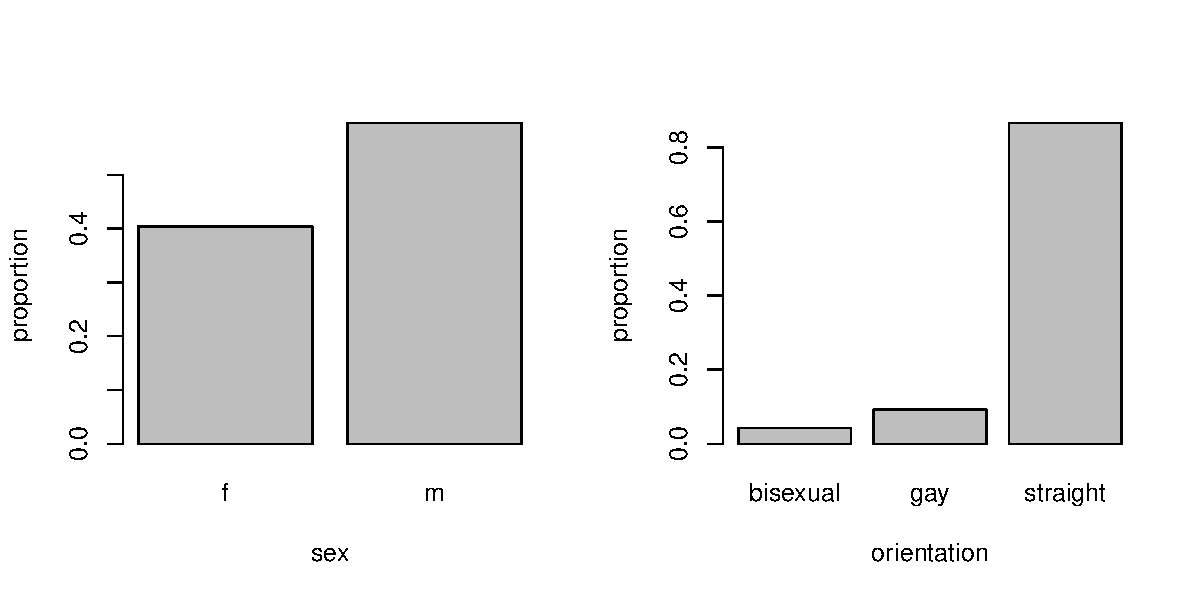
\includegraphics[width=\maxwidth]{figure/sex_and_orientation-1} 

}

\caption[Distributions of sex and sexual orientation]{Distributions of sex and sexual orientation.}\label{fig:sex_and_orientation}
\end{figure}


\end{knitrout}

However, in order to accurately portray the dating landscape we can't just consider the \textbf{marginal distributions} of these variables, we must consider their \textbf{joint} and \textbf{conditional distributions} i.e. their cross-classifications.  We describe the distribution of ``sexual orientation'' conditional on ``sex.''  For example, of all females (the condition) what proportion are bisexual?  We do this using the \verb#tally()# command from the \verb#mosaic# package.  Furthermore, we visualize their joint distribution, as represented by a contingency table, via the mosaicplot shown in Figure \ref{fig:sex_by_orientation}.

\begin{knitrout}
\definecolor{shadecolor}{rgb}{0.969, 0.969, 0.969}\color{fgcolor}\begin{kframe}
\begin{alltt}
\hlkwd{tally}\hlstd{(orientation} \hlopt{~} \hlstd{sex, profiles,} \hlkwc{format}\hlstd{=}\hlstr{'proportion'}\hlstd{)}
\end{alltt}
\begin{verbatim}
##            sex
## orientation     f     m
##    bisexual 0.083 0.022
##    gay      0.066 0.111
##    straight 0.851 0.867
\end{verbatim}
\begin{alltt}
\hlstd{sex.by.orientation} \hlkwb{<-} \hlkwd{with}\hlstd{(profiles,} \hlkwd{table}\hlstd{(sex, orientation))}
\hlstd{sex.by.orientation}
\end{alltt}
\begin{verbatim}
##    orientation
## sex bisexual   gay straight
##   f     1996  1588    20533
##   m      771  3985    31073
\end{verbatim}
\begin{alltt}
\hlkwd{mosaicplot}\hlstd{(sex.by.orientation}\hlopt{/}\hlstd{n,} \hlkwc{main}\hlstd{=}\hlstr{"Sex vs Orientation"}\hlstd{)}
\end{alltt}
\end{kframe}\begin{figure}

{\centering 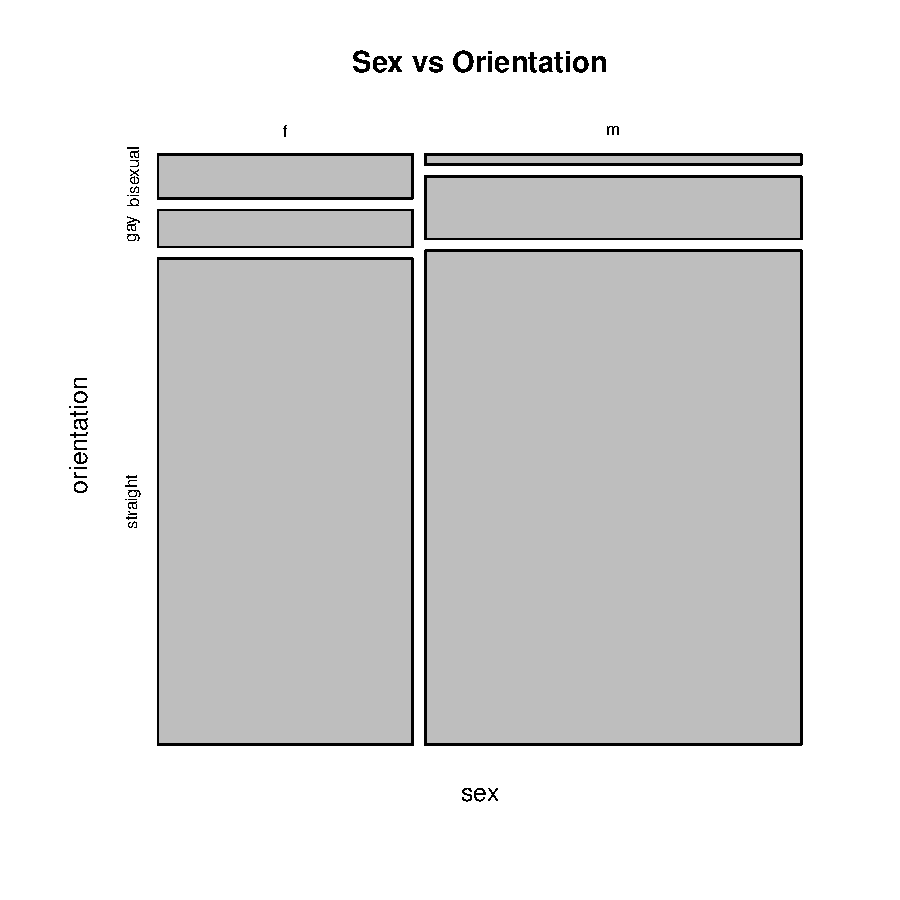
\includegraphics[width=\maxwidth]{figure/sex_by_orientation-1} 

}

\caption[Cross-classification of sex and sexual orientation]{Cross-classification of sex and sexual orientation.}\label{fig:sex_by_orientation}
\end{figure}


\end{knitrout}

%We proceed with a \textit{chi-square tests for independence} between these two variables, performing one using the \verb#chisq.test()# command.
%<<cache=TRUE>>=
%chisq.test(sex.by.orientation)
%@



\subsubsection{Pedagogical Discussion}
This exercise was an opportunity to concretize the statistical notions such as marginal/joint/conditional distributions and sampling bias.  The data indicate that the San Francisco OkCupid dating population skews male and while the proportions of males and females who list themselves as straight are similar, a higher proportion of males list themselves as gay while a higher proportion of females list themselves as bisexual.  Many students were not surprised by this fact as they were well aware of the gender imbalance issues in the large technology sector in the San Francisco Bay Area and San Francisco's history of being a bastion for the gay community.  An interesting discussion arose on the sociological factors in why more women listed themselves as bisexual then men; this topic has previously been covered on the blog OkTrends\cite{OkTrendsLies}.

The question of generalizability was presented in an introductory probability and statistics class homework.  Almost all students were able to recognize the selection biases of who signs up for this site and hence the non-generalizability of the results.  For example some recognized that OkCupid's demographic is most likely different than other dating website demographics such as \url{match.com} (which is not free) or \url{christiansingles.com} (which is targeted towards Christians).  So while 59946 users may initially seem like a fairly large sample, we emphasized that ``bigger'' isn't always ``better'' when it comes to obtaining generalizable results due to the aforementioned selection biases.  This proved an excellent segue to discussions on John Tukey's famous quote about the sexologist Alfred Kinsey ``A random selection of three people would have been better than a group of 300 chosen by Mr. Kinsey'' and Kate Crawford of Microsoft Research's YouTube talk ``Algorithmic Illusions: Hidden Biases of Big Data''~\cite{Strata}.

Further questions one can pose to students include ``Which dating demographic would you say has it the best and worst in terms of our simplified categorization?'', ``What variable do you think should be incorporated next in order to faithfully represent the OkCupid dating pool?'',  and ``Even though not perfectly generalizable, to what degree can we apply these results to, for example, New York OkCupid users?''.







%---------------------------------------------------------------
\subsection{Text Analysis}\label{essays}
%---------------------------------------------------------------
\subsubsection{Exercise}
The next exercise focuses on the responses to the essay questions, providing an opportunity to perform text analysis.  Words are also called ``strings'' in the context of computer programming.  Manipulating text data in R is often a complicated affair, so we present some code that is at an intermediate level to preprocess the essay responses for analysis.  In order to output a single vector \verb#essays# that contains all 10 essay responses for each user concatenated together, the following code:

\begin{itemize}
\item Uses the \verb#select()# command from the \verb#dplyr# package to select the 10 essay columns as identified by the fact they \verb#starts_with("essay")#.
\item Converts the essays from list to matrix format with 10 columns.
\item For each user concatenates the 10 columns to form a single character string.  The code applies the function \verb#paste(x, collapse=" ")# to every essay where \verb#x# is a user's set of 10 essay responses, and the \verb#paste()# function collapses \verb#x# across columns while separating the elements by a space.  We do this for each set of essays (i.e. each row of \verb#essays#) via the \verb#apply()# command and setting the second argument to \verb#1#.
\item Replace all HTML line breaks (\verb#\n#) and paragraph breaks (\verb#<br />#) with spaces as well to make the outputs more readable.
\end{itemize}

\begin{knitrout}
\definecolor{shadecolor}{rgb}{0.969, 0.969, 0.969}\color{fgcolor}\begin{kframe}
\begin{alltt}
\hlstd{essays} \hlkwb{<-} \hlkwd{select}\hlstd{(profiles,} \hlkwd{starts_with}\hlstd{(}\hlstr{"essay"}\hlstd{))}
\hlstd{essays} \hlkwb{<-} \hlkwd{apply}\hlstd{(essays,} \hlnum{1}\hlstd{, paste,} \hlkwc{collapse}\hlstd{=}\hlstr{" "}\hlstd{)}
\hlstd{essays} \hlkwb{<-} \hlkwd{str_replace_all}\hlstd{(essays,} \hlstr{"\textbackslash{}n"}\hlstd{,} \hlstr{" "}\hlstd{)}
\hlstd{essays} \hlkwb{<-} \hlkwd{str_replace_all}\hlstd{(essays,} \hlstr{"<br />"}\hlstd{,} \hlstr{" "}\hlstd{)}
\end{alltt}
\end{kframe}
\end{knitrout}

We ask:  Do male and female OkCupid users use words at different rates in their essay responses?  We search for the presence of a word in a user's essays using the  \verb#str_detect()# command in the \verb#stringr# package.  We then use the \verb#tally()# illustrated in Section \ref{sex_by_sexual_orientation} to compute the distribution conditional on sex.  For example, the word ``book'' is used by 62\% of female profiles and 55\% of male profiles.  In Table \ref{tab:word_use} we make similar comparisons for the use of the words ``travel'', ``food'', ``wine'', and ``beer.''

\begin{knitrout}
\definecolor{shadecolor}{rgb}{0.969, 0.969, 0.969}\color{fgcolor}\begin{kframe}
\begin{alltt}
\hlstd{profiles}\hlopt{$}\hlstd{has.book} \hlkwb{<-} \hlkwd{str_detect}\hlstd{(essays,} \hlstr{"book"}\hlstd{)}
\hlkwd{tally}\hlstd{(has.book} \hlopt{~} \hlstd{sex, profiles,} \hlkwc{format}\hlstd{=}\hlstr{'proportion'}\hlstd{)}
\end{alltt}
\begin{verbatim}
##         sex
## has.book    f    m
##    TRUE  0.62 0.55
##    FALSE 0.38 0.45
\end{verbatim}
\end{kframe}
\end{knitrout}

% latex table generated in R 3.1.2 by xtable 1.7-4 package
% Sat Apr  4 15:07:22 2015
\begin{table}[ht]
\centering
\begin{tabular}{lrr}
  \hline
word & female & male \\ 
  \hline
travel & 0.386 & 0.299 \\ 
  food & 0.652 & 0.601 \\ 
  wine & 0.201 & 0.117 \\ 
  beer & 0.087 & 0.109 \\ 
   \hline
\end{tabular}
\caption{Proportions of each sex using word in essays.} 
\label{tab:word_use}
\end{table}


We also verify the co-occurrence of words, such as ``wine'' and ``travel'', visualizing their relationship in a mosaicplot in Figure \ref{fig:travel_vs_wine}.

\begin{knitrout}
\definecolor{shadecolor}{rgb}{0.969, 0.969, 0.969}\color{fgcolor}\begin{kframe}
\begin{alltt}
\hlstd{profiles}\hlopt{$}\hlstd{has.wine} \hlkwb{<-} \hlkwd{str_detect}\hlstd{(essays,} \hlstr{"wine"}\hlstd{)}
\hlstd{profiles}\hlopt{$}\hlstd{has.travel} \hlkwb{<-} \hlkwd{str_detect}\hlstd{(essays,} \hlstr{"travel"}\hlstd{)}
\hlstd{travel.vs.wine} \hlkwb{<-} \hlkwd{tally}\hlstd{(}\hlopt{~}\hlstd{has.travel} \hlopt{+} \hlstd{has.wine,} \hlkwc{data}\hlstd{=profiles)}
\hlkwd{mosaicplot}\hlstd{(travel.vs.wine,} \hlkwc{main}\hlstd{=}\hlstr{""}\hlstd{,} \hlkwc{xlab}\hlstd{=}\hlstr{"travel"}\hlstd{,} \hlkwc{ylab}\hlstd{=}\hlstr{"wine"}\hlstd{)}
\end{alltt}
\end{kframe}\begin{figure}

{\centering 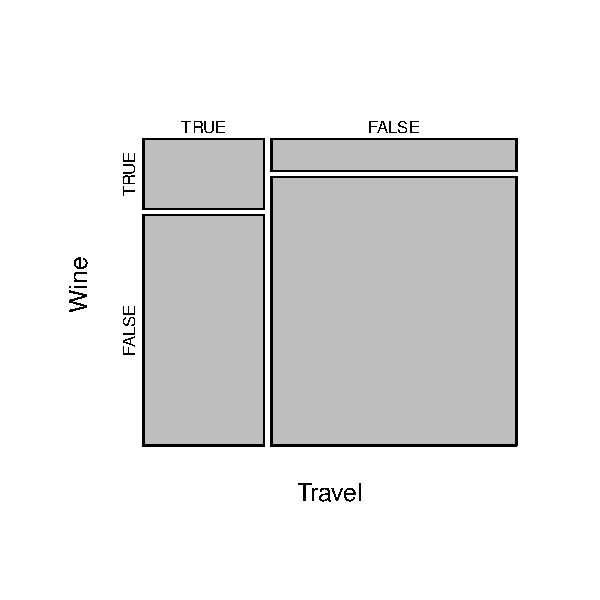
\includegraphics[width=\maxwidth]{figure/travel_vs_wine-1} 

}

\caption[Co-occurrence of `travel' and `wine]{Co-occurrence of `travel' and `wine.'}\label{fig:travel_vs_wine}
\end{figure}


\end{knitrout}

We evaluate the statistical significance of the difference in the use of the word ``football'' via a two-sample proportions test using the \verb#prop.test()# function where you specify vectors \verb#x# of the successes of each group and \verb#n# of the numbers in each group.  While the difference of around 0.5\% is statistically significant for almost any $\alpha$-level, it can be argued that this difference is of little practical significance.

\begin{knitrout}
\definecolor{shadecolor}{rgb}{0.969, 0.969, 0.969}\color{fgcolor}\begin{kframe}
\begin{alltt}
\hlstd{profiles}\hlopt{$}\hlstd{has.football} \hlkwb{<-} \hlkwd{str_detect}\hlstd{(essays,} \hlstr{"football"}\hlstd{)}
\hlstd{results} \hlkwb{<-} \hlkwd{table}\hlstd{(profiles}\hlopt{$}\hlstd{has.football, profiles}\hlopt{$}\hlstd{sex)}
\hlkwd{prop.test}\hlstd{(}\hlkwc{x}\hlstd{=results[}\hlnum{2}\hlstd{, ],} \hlkwc{n}\hlstd{=}\hlkwd{colSums}\hlstd{(results),} \hlkwc{alternative}\hlstd{=}\hlstr{"two.sided"}\hlstd{)}
\end{alltt}
\begin{verbatim}
## 
## 	2-sample test for equality of proportions with continuity
## 	correction
## 
## data:  x and n
## X-squared = 13, df = 1, p-value = 0.0002929
## alternative hypothesis: two.sided
## 95 percent confidence interval:
##  -0.0085 -0.0026
## sample estimates:
## prop 1 prop 2 
##  0.031  0.036
\end{verbatim}
\end{kframe}
\end{knitrout}

And finally, consider the following fun exercise: we generate the top 500 words used by males and females respectively.  The following code uses the ``pipe'' \verb#%>%# operator from the \verb#dplyr# package to send the output of one function into the next function wherever the period is located.  For example, the following two lines of code perform the identical task:

\begin{knitrout}
\definecolor{shadecolor}{rgb}{0.969, 0.969, 0.969}\color{fgcolor}\begin{kframe}
\begin{alltt}
\hlkwd{c}\hlstd{(}\hlnum{1}\hlstd{,} \hlnum{2}\hlstd{,} \hlnum{3}\hlstd{,} \hlnum{4}\hlstd{)} \hlopt \hlkwd{sum}\hlstd{(.)}
\hlkwd{sum}\hlstd{(}\hlkwd{c}\hlstd{(}\hlnum{1}\hlstd{,} \hlnum{2}\hlstd{,} \hlnum{3}\hlstd{,} \hlnum{4}\hlstd{))}
\end{alltt}
\end{kframe}
\end{knitrout}

This allows us to avoid having multiple R functions nested in a large number of parentheses and highlights the sequence of commands performed.  In our case, the code below:

\begin{itemize}
\item Pulls the \verb#subset# of \verb#essays# corresponding to males and females.
\item Splits up the each user's essay text at each space, i.e. cuts it up into words, using the \verb#str_split()# command from the \verb#stringr# package.
\item Converts the list of words into a vector of words.
\item Computes the frequency table using the \verb#table()# command.
\item Sorts them in decreasing order.
\item Extracts the words (and not the frequency counts), which are the \verb#names# of each element of the vector.
\end{itemize}

\begin{knitrout}
\definecolor{shadecolor}{rgb}{0.969, 0.969, 0.969}\color{fgcolor}\begin{kframe}
\begin{alltt}
\hlstd{male.words} \hlkwb{<-} \hlkwd{subset}\hlstd{(essays, profiles}\hlopt{$}\hlstd{sex} \hlopt{==} \hlstr{"m"}\hlstd{)} \hlopt \hlkwd{str_split}\hlstd{(.,} \hlstr{" "}\hlstd{)} \hlopt \hlkwd{unlist}\hlstd{(.)} \hlopt
  \hlkwd{table}\hlstd{(.)} \hlopt \hlkwd{sort}\hlstd{(.,} \hlkwc{decreasing}\hlstd{=}\hlnum{TRUE}\hlstd{)} \hlopt \hlkwd{names}\hlstd{(.)}
\hlstd{female.words} \hlkwb{<-} \hlkwd{subset}\hlstd{(essays, profiles}\hlopt{$}\hlstd{sex} \hlopt{==} \hlstr{"f"}\hlstd{)} \hlopt \hlkwd{str_split}\hlstd{(.,} \hlstr{" "}\hlstd{)} \hlopt \hlkwd{unlist}\hlstd{(.)} \hlopt
  \hlkwd{table}\hlstd{(.)} \hlopt \hlkwd{sort}\hlstd{(.,} \hlkwc{decreasing}\hlstd{=}\hlnum{TRUE}\hlstd{)} \hlopt \hlkwd{names}\hlstd{(.)}
\end{alltt}
\end{kframe}
\end{knitrout}

However, for both males and females, the top words are not interesting (as reflected by the top 25 below), as they include many particles such as ``I'', ``and'', and ``the.''  Therefore, we consider the top 500 words used by males \textit{that are not in the top 500 words used by females}, and vice-versa, by taking the difference in sets using the \verb#setdiff()# command.
\begin{knitrout}
\definecolor{shadecolor}{rgb}{0.969, 0.969, 0.969}\color{fgcolor}\begin{kframe}
\begin{alltt}
\hlcom{# Top 25 male words:}
\hlstd{male.words[}\hlnum{1}\hlopt{:}\hlnum{25}\hlstd{]}
\end{alltt}
\begin{verbatim}
##  [1] ""                "i"               "and"            
##  [4] "the"             "to"              "a"              
##  [7] "of"              "my"              "in"             
## [10] "i'm"             "you"             "for"            
## [13] "with"            "that"            "is"             
## [16] "have"            "like"            "on"             
## [19] "but"             "or"              "<a"             
## [22] "at"              "class=\"ilink\"" "it"             
## [25] "am"
\end{verbatim}
\begin{alltt}
\hlcom{# Top 25 female words}
\hlstd{female.words[}\hlnum{1}\hlopt{:}\hlnum{25}\hlstd{]}
\end{alltt}
\begin{verbatim}
##  [1] ""     "i"    "and"  "the"  "to"   "a"    "my"   "of"   "in"   "i'm" 
## [11] "with" "for"  "you"  "that" "have" "is"   "love" "am"   "but"  "like"
## [21] "or"   "on"   "at"   "it"   "be"
\end{verbatim}
\begin{alltt}
\hlcom{# Words in the males top 500 that weren't in the females' top 500:}
\hlkwd{setdiff}\hlstd{(male.words[}\hlnum{1}\hlopt{:}\hlnum{500}\hlstd{], female.words[}\hlnum{1}\hlopt{:}\hlnum{500}\hlstd{])}
\end{alltt}
\begin{verbatim}
##  [1] ","         "video"     "company"   "sports"    "/"        
##  [6] "internet"  "future"    "computer"  "star"      "well,"    
## [11] "well."     "away"      "john"      "until"     "business" 
## [16] "us"        "type"      "couple"    "generally" "2"        
## [21] "more."     "went"      "bar"       "science"   "woman"    
## [26] "work."     "started"   "does"      "here."     "found"    
## [31] "three"     "lost"      "means"     "do."       "become"   
## [36] "run"       "that,"
\end{verbatim}
\begin{alltt}
\hlcom{# Words in the male top 500 that weren't in the females' top 500:}
\hlkwd{setdiff}\hlstd{(female.words[}\hlnum{1}\hlopt{:}\hlnum{500}\hlstd{], male.words[}\hlnum{1}\hlopt{:}\hlnum{500}\hlstd{])}
\end{alltt}
\begin{verbatim}
##  [1] "loving"      "dancing,"    "love,"       "appreciate"  "dog"        
##  [6] "hair"        "beautiful"   "laughing"    "passionate"  "red"        
## [11] "cooking,"    ";)"          "laugh."      "please"      "kids"       
## [16] "local"       "drinking"    "kinds"       "family."     "healthy"    
## [21] "adventure"   "explore"     "laugh,"      "men"         "smile."     
## [26] "comfortable" "crazy"       "nature"      "hiking,"     "day."       
## [31] "chocolate"   "huge"        "change"      "dating"      "sex"        
## [36] "met"         "movies."
\end{verbatim}
\end{kframe}
\end{knitrout}




\subsubsection{Teaching Goals and Discussions}
This exercise provides students with experience performing basic text processing, mining, and analysis.  Given the more advanced tools used in the last component of the exercise (the top words used by males and females), we suggest this be reserved for students with more familiarity with R.  We deliberately did not pre-process the data for students to remove punctuation and HTML tags to both to keep the code simple and to demonstrate the reality to students that ``real'' data is often very messy, requiring significant work to clean up.

Statistical concepts include the difference between practical and statistical significance as demonstrated by the difference in proportion of males and females that used the word ``football''.  This can lead to discussions of what it means to conduct hypothesis tests when the sample size is as large as 59946.  Furthermore, simple comparisons via basic set operations can be very powerful tools yielding valuable insight.  For example, the difference in lengths of words and number of adjective used between males and females in our surface-level analysis is striking.

The richness of the essay data allows for students to verify and challenge prior sociological beliefs and preconceptions using empirical data.  Furthermore, such analyses can expose and confront students with biases, prejudices, and behaviors that they didn't even know they hold or exhibit.

Another interesting investigation for students to pursue is to what degree do the above results hold when the groups we are comparing are further refined (grouping by sex \textit{and} sexual orientation for example).  Even bolder goals include introducing text analysis concepts such as regular expressions, inverse document frequency, natural language processing, and Latent Dirichlet analysis\cite{LDA:2003}.







%---------------------------------------------------------------
\subsection{Predictors of Sex}
%---------------------------------------------------------------
The final exercise provides an opportunity to fit a predictive model for sex using logistic regression.  In order to reinforce the concepts of logistic regression, we keep things simple and consider only one predictor variable in the logistic model: height.  We restrict to only those users whose heights are reasonable as defined previously in Section \ref{section_height} and take a sample of size 5995 (10\% of the data) to speed up computation using the \verb#sample_n()# command from the \verb#dplyr# package.

\begin{knitrout}
\definecolor{shadecolor}{rgb}{0.969, 0.969, 0.969}\color{fgcolor}\begin{kframe}
\begin{alltt}
\hlstd{profiles} \hlkwb{<-} \hlkwd{filter}\hlstd{(profiles, height}\hlopt{>=}\hlnum{55} \hlopt{&} \hlstd{height} \hlopt{<=}\hlnum{80}\hlstd{)}
\hlstd{profiles} \hlkwb{<-} \hlkwd{sample_n}\hlstd{(profiles,} \hlnum{5995}\hlstd{)}
\end{alltt}
\end{kframe}
\end{knitrout}

\subsubsection{Exercise}
We convert the \verb#sex# variable to a binary \verb#is.female# variable, where \verb#1# if female and \verb#0# if male, using the \verb#ifelse()# function.  We plot the points as in Figure \ref{fig:is_female_vs_height}, making use of the \verb#ggplot2# package.

\begin{knitrout}
\definecolor{shadecolor}{rgb}{0.969, 0.969, 0.969}\color{fgcolor}\begin{kframe}
\begin{alltt}
\hlstd{profiles}\hlopt{$}\hlstd{is.female} \hlkwb{=} \hlkwd{ifelse}\hlstd{(profiles}\hlopt{$}\hlstd{sex}\hlopt{==}\hlstr{"f"}\hlstd{,} \hlnum{1}\hlstd{,} \hlnum{0}\hlstd{)}
\hlkwd{ggplot}\hlstd{(}\hlkwc{data}\hlstd{=profiles,} \hlkwd{aes}\hlstd{(}\hlkwc{x}\hlstd{=height,} \hlkwc{y}\hlstd{=is.female))} \hlopt{+} \hlkwd{geom_point}\hlstd{()} \hlopt{+}
  \hlkwd{xlab}\hlstd{(}\hlstr{"Height (in.)"}\hlstd{)} \hlopt{+} \hlkwd{ylab}\hlstd{(}\hlstr{"Is female?"}\hlstd{)}
\end{alltt}
\end{kframe}\begin{figure}

{\centering 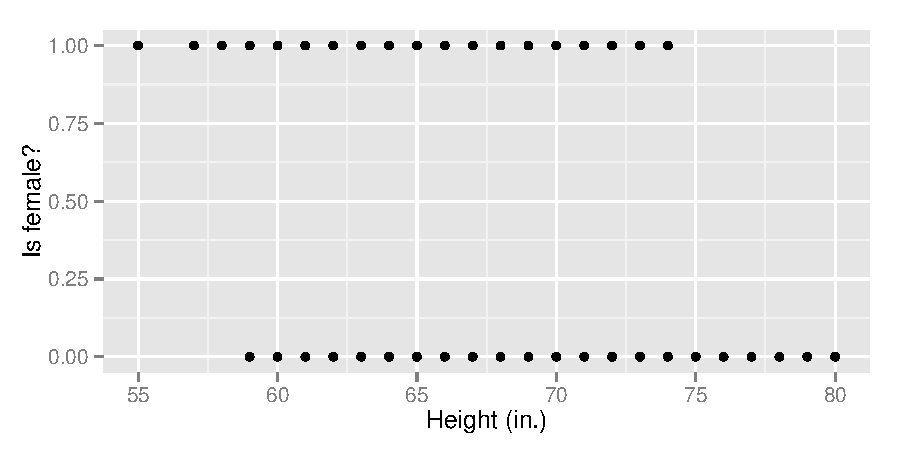
\includegraphics[width=\maxwidth]{figure/is_female_vs_height-1} 

}

\caption[Female indicator vs height]{Female indicator vs height.}\label{fig:is_female_vs_height}
\end{figure}


\end{knitrout}

This plot is not very useful, as the overlap of the points makes it difficult for determine how many points are involved.  We use the \verb#jitter()# function to add a little random noise to each clump of points as shown in Figure \ref{fig:is_female_vs_height_jittered}.

\begin{knitrout}
\definecolor{shadecolor}{rgb}{0.969, 0.969, 0.969}\color{fgcolor}\begin{kframe}
\begin{alltt}
\hlkwd{ggplot}\hlstd{(}\hlkwc{data}\hlstd{=profiles,} \hlkwd{aes}\hlstd{(}\hlkwc{x}\hlstd{=}\hlkwd{jitter}\hlstd{(height),} \hlkwc{y}\hlstd{=}\hlkwd{jitter}\hlstd{(is.female)))} \hlopt{+}
  \hlkwd{geom_point}\hlstd{()} \hlopt{+} \hlkwd{xlab}\hlstd{(}\hlstr{"Height (in.)"}\hlstd{)} \hlopt{+} \hlkwd{ylab}\hlstd{(}\hlstr{"Is female?"}\hlstd{)}
\end{alltt}
\end{kframe}\begin{figure}

{\centering \includegraphics[width=\maxwidth]{figure/is_female_vs_height_jittered-1} 

}

\caption[Female indicator vs height (jittered)]{Female indicator vs height (jittered).}\label{fig:is_female_vs_height_jittered}
\end{figure}


\end{knitrout}

We fit both linear and logistic regression models using height as the sole predictor.  In order to summarize the results, we use the \verb#msummary()# from the \verb#mosaic# package as its output is much more digestible than the output of the standard \verb#summary()# command.  Furthermore, we extract the coefficients of the linear model using the \verb#coef()# command.

\begin{knitrout}
\definecolor{shadecolor}{rgb}{0.969, 0.969, 0.969}\color{fgcolor}\begin{kframe}
\begin{alltt}
\hlstd{linear.model} \hlkwb{<-} \hlkwd{lm}\hlstd{(is.female} \hlopt{~} \hlstd{height,} \hlkwc{data}\hlstd{=profiles)}
\hlkwd{msummary}\hlstd{(linear.model)}
\end{alltt}
\begin{verbatim}
##             Estimate Std. Error t value Pr(>|t|)    
## (Intercept)  6.42887    0.08373    76.8   <2e-16 ***
## height      -0.08831    0.00122   -72.1   <2e-16 ***
## 
## Residual standard error: 0.36 on 5993 degrees of freedom
## Multiple R-squared:  0.465,	Adjusted R-squared:  0.464 
## F-statistic: 5.2e+03 on 1 and 5993 DF,  p-value: <2e-16
\end{verbatim}
\begin{alltt}
\hlstd{b1} \hlkwb{<-} \hlkwd{coef}\hlstd{(linear.model)}
\hlstd{b1}
\end{alltt}
\begin{verbatim}
## (Intercept)      height 
##       6.429      -0.088
\end{verbatim}
\end{kframe}
\end{knitrout}

\begin{knitrout}
\definecolor{shadecolor}{rgb}{0.969, 0.969, 0.969}\color{fgcolor}\begin{kframe}
\begin{alltt}
\hlstd{logistic.model} \hlkwb{<-} \hlkwd{glm}\hlstd{(is.female} \hlopt{~} \hlstd{height,} \hlkwc{family}\hlstd{=binomial,} \hlkwc{data}\hlstd{=profiles)}
\hlkwd{msummary}\hlstd{(logistic.model)}
\end{alltt}
\begin{verbatim}
## Coefficients:
##             Estimate Std. Error z value Pr(>|z|)    
## (Intercept)  44.9999     1.1374    39.6   <2e-16 ***
## height       -0.6705     0.0169   -39.8   <2e-16 ***
## 
## (Dispersion parameter for binomial family taken to be 1)
## 
##     Null deviance: 8075.1  on 5994  degrees of freedom
## Residual deviance: 4460.2  on 5993  degrees of freedom
## AIC: 4464
## 
## Number of Fisher Scoring iterations: 6
\end{verbatim}
\begin{alltt}
\hlstd{b2} \hlkwb{<-} \hlkwd{coefficients}\hlstd{(logistic.model)}
\hlstd{b2}
\end{alltt}
\begin{verbatim}
## (Intercept)      height 
##       45.00       -0.67
\end{verbatim}
\end{kframe}
\end{knitrout}

In both cases, we observe that the coefficient associated with height is negative, in other words, as height increases, the fitted probability of being female decreases.  However the interpretability of the logistic model is difficult.  We thus plot both regressions lines in Figure \ref{fig:is_female_vs_height_logistic_vs_linear}, with the linear regression in red and the logistic regression in blue.  The latter necessitates the function \verb#inverse.logit()# in order to compute the inverse logit of the linear equation to obtain the fitted probabilities $\widehat{p}_i$:

\[
\widehat{p}_i = \frac{1}{1+\exp\left(-(\widehat{\beta}_0 + \widehat{\beta}_1 \times \mbox{height}_i)\right)}
\]


\begin{knitrout}
\definecolor{shadecolor}{rgb}{0.969, 0.969, 0.969}\color{fgcolor}\begin{kframe}
\begin{alltt}
\hlstd{inverse.logit} \hlkwb{<-} \hlkwa{function}\hlstd{(}\hlkwc{x}\hlstd{,} \hlkwc{b}\hlstd{)\{}
  \hlstd{linear.equation} \hlkwb{<-} \hlstd{b[}\hlnum{1}\hlstd{]} \hlopt{+} \hlstd{b[}\hlnum{2}\hlstd{]}\hlopt{*}\hlstd{x}
  \hlnum{1}\hlopt{/}\hlstd{(}\hlnum{1}\hlopt{+}\hlkwd{exp}\hlstd{(}\hlopt{-}\hlstd{linear.equation))}
\hlstd{\}}
\hlkwd{ggplot}\hlstd{(}\hlkwc{data}\hlstd{=profiles,} \hlkwd{aes}\hlstd{(}\hlkwc{x}\hlstd{=}\hlkwd{jitter}\hlstd{(height),} \hlkwc{y}\hlstd{=}\hlkwd{jitter}\hlstd{(is.female)))} \hlopt{+}
  \hlkwd{geom_point}\hlstd{()} \hlopt{+} \hlkwd{xlab}\hlstd{(}\hlstr{"Height (in.)"}\hlstd{)} \hlopt{+} \hlkwd{ylab}\hlstd{(}\hlstr{"Is female?"}\hlstd{)} \hlopt{+}
  \hlkwd{geom_abline}\hlstd{(}\hlkwc{intercept}\hlstd{=b1[}\hlnum{1}\hlstd{],} \hlkwc{slope}\hlstd{=b1[}\hlnum{2}\hlstd{],} \hlkwc{col}\hlstd{=}\hlstr{"red"}\hlstd{,} \hlkwc{size}\hlstd{=}\hlnum{2}\hlstd{)} \hlopt{+}
  \hlkwd{stat_function}\hlstd{(}\hlkwc{fun} \hlstd{= inverse.logit,} \hlkwc{args}\hlstd{=}\hlkwd{list}\hlstd{(}\hlkwc{b}\hlstd{=b2),} \hlkwc{color}\hlstd{=}\hlstr{"blue"}\hlstd{,} \hlkwc{size}\hlstd{=}\hlnum{2}\hlstd{)}
\end{alltt}
\end{kframe}\begin{figure}

{\centering \includegraphics[width=\maxwidth]{figure/is_female_vs_height_logistic_vs_linear-1} 

}

\caption[Linear and logistic regression curves]{Linear and logistic regression curves.}\label{fig:is_female_vs_height_logistic_vs_linear}
\end{figure}


\end{knitrout}

We observe that linear regression (red curve) yields fitted probabilities less than 0 for heights less than 61 inches for and fitted probabilities greater than 1 for heights over 73 inches, which do not make sense.  This is not a problem with logistic regression as the shape of the logistic curve ensures fitted probabilities are between 0 and 1 for all heights.   We therefore deem logistic regression to be a more appropriate technique for this data than simple linear regression.

However, when predicting a user's gender, just using the fitted probabilities $\widehat{p}_i$ are insufficient; a decision threshold is necessary.  In other words, a point at which if the probability of being female is exceeded, we \textit{declare} that user to be female.  Looking at the histogram of fitted probabilities, we pick an appropriate decision threshold $p^*$ such that for all users who's $\widehat{p}_i > p^*$ we predict the user to be female.  We opt for $p^* = 0.5$ and highlight this in red in Figure \ref{fig:fitted_values}.  In order to evaluate the performance of our model and our decision threshold, we produce the contingency table comparing the true and predicted values.

\begin{knitrout}
\definecolor{shadecolor}{rgb}{0.969, 0.969, 0.969}\color{fgcolor}\begin{kframe}
\begin{alltt}
\hlstd{profiles}\hlopt{$}\hlstd{p.hat} \hlkwb{<-} \hlkwd{fitted}\hlstd{(logistic.model)}
\hlkwd{hist}\hlstd{(profiles}\hlopt{$}\hlstd{p.hat,} \hlkwc{xlab}\hlstd{=}\hlstr{"p.hat"}\hlstd{,} \hlkwc{main}\hlstd{=}\hlstr{""}\hlstd{)}
\hlkwd{abline}\hlstd{(}\hlkwc{v}\hlstd{=}\hlnum{0.5}\hlstd{,} \hlkwc{col}\hlstd{=}\hlstr{"red"}\hlstd{,} \hlkwc{lwd}\hlstd{=}\hlnum{2}\hlstd{)}
\end{alltt}
\end{kframe}\begin{figure}

{\centering 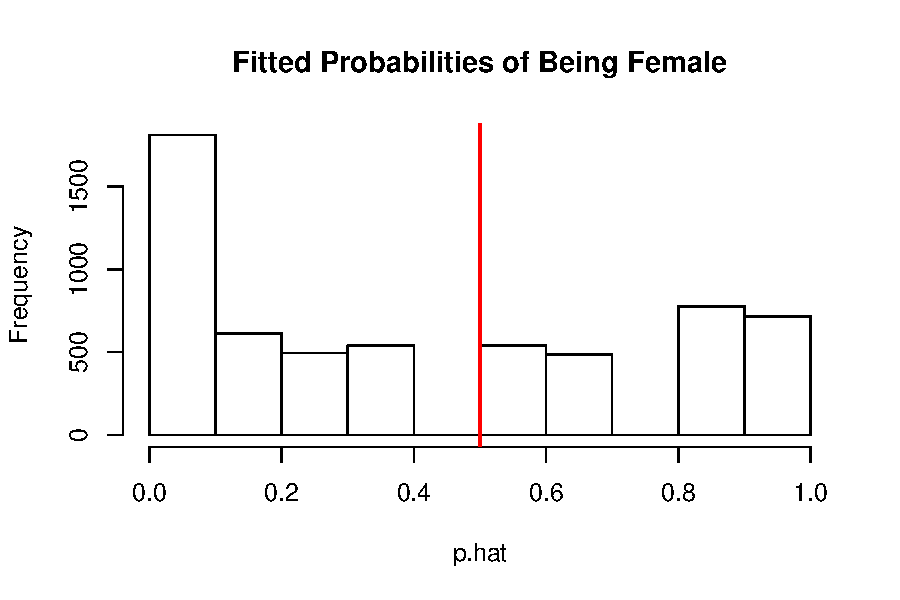
\includegraphics[width=\maxwidth]{figure/fitted_values-1} 

}

\caption[Fitted probabilities of being female and decision threshold (in red)]{Fitted probabilities of being female and decision threshold (in red).}\label{fig:fitted_values}
\end{figure}

\begin{kframe}\begin{alltt}
\hlstd{profiles}\hlopt{$}\hlstd{predicted.female} \hlkwb{<-} \hlstd{profiles}\hlopt{$}\hlstd{p.hat} \hlopt{>=} \hlnum{0.5}
\hlkwd{table}\hlstd{(}\hlkwc{truth}\hlstd{=profiles}\hlopt{$}\hlstd{is.female,} \hlkwc{prediction}\hlstd{=profiles}\hlopt{$}\hlstd{predicted.female)}
\end{alltt}
\begin{verbatim}
##      prediction
## truth FALSE TRUE
##     0  3024  566
##     1   452 1953
\end{verbatim}
\end{kframe}
\end{knitrout}



\subsubsection{Pedagogical Discussion}
We find that the jump from linear to logistic regression is hard for many students to grasp at first.  For example, students often ask ``Why the $\log$ and $\exp$ functions?'' and ``So we are not modelling the outcome variable $Y_i$, we're modeling the probability $p_i$ that $Y_i$ equals 1?''  This exercise allows students to build up to the notion of logistic regression from the ground up using data visualizations.  We also argue that on top of fitting the model and interpreting any results, students should also use the results to make explicit predictions and evaluate the logistic model's predictive power.  We ask the students ``For what proportion of people did you guess wrong'' referring to the misclassification error rate, in this case 16.98\%.  Also solving for height using $p^*=0.5$ yields a height of 67.11 inches, corresponding to 5 foot 7 inches, which is the smallest height in Figure \ref{fig:heights_by_sex} at which the proportion of males starts to exceed the proportion of females.  This point can be highlighted to students, tying together the exercise in Section \ref{section_height} to this one.

Further questions to ask of students include building a model with more than one predictor, incorporating essay information from Section \ref{essays}, evaluating the \textit{false positive rate} (the proportion of users who were predicted to be female who were actually male), evaluating the \textit{false negative rate} (the proportion of user's who were predicted to be male who were actually female), and varying the decision threshold $p^*$.












%------------------------------------------------------------------------------
%
\section{Conclusions}
%
%------------------------------------------------------------------------------
We feel that this dataset is an ideal one for use in introductory statistics and data science classes as the salience of the dataset provides students with an interesting vehicle for learning important concepts.  By presenting questions to students that allow for the use of background knowledge of the problem, whether it be the news, stereotypes, sociological knowledge, students are much better primed to absorb statistical lessons.  Furthermore,

\begin{enumerate}
\item The data consists of a rich array of categorical, ordinal, numerical, and text variables.
\item This is an instance of real data that is messy, requires much data manipulation, has many suspicious values, and includes categorical variables of a complicated nature (for instance, there are 218 unique responses to the ethnicity variable).  This reinforces to students that time and energy must be often invested into preparing the data for analysis.
\item The dataset is of modest size.  While $n = 59946$ is not an overwhelmingly large number of observations, it is still much larger than typical datasets used in many introductory probability and statistics classes.
\end{enumerate}

All the files, including the original data and the R Sweave \verb#.Rmd# file used to create this document, can be found at \url{https://github.com/rudeboybert/JSE_OkCupid}.  Note that the file \verb#profiles.csv.zip# must be unzipped first.  All R code used in this document can be outputted into an R script file by using the \verb#purl()# command in the \verb#knitr# package on the \verb#JSE.Rnw# R Sweave document.
\begin{knitrout}
\definecolor{shadecolor}{rgb}{0.969, 0.969, 0.969}\color{fgcolor}\begin{kframe}
\begin{alltt}
\hlkwd{purl}\hlstd{(}\hlkwc{input}\hlstd{=}\hlstr{"JSE.Rnw"}\hlstd{,} \hlkwc{output}\hlstd{=}\hlstr{"JSE.R"}\hlstd{,} \hlkwc{quiet}\hlstd{=}\hlnum{TRUE}\hlstd{)}
\end{alltt}
\end{kframe}
\end{knitrout}










%------------------------------------------------------------------------------
%
\section{Acknowledgements}\label{ack}
%
%------------------------------------------------------------------------------
First, we thank OkCupid President and co-founder Christian Rudder for agreeing to our use of this dataset (under the condition that the dataset remains public).  Second, we thank Everett Wetchler of Bayes Impact \url{everett.wetchler@gmail.com} for providing the data; the python script used to scrape the data can be found at \url{https://github.com/evee746/okcupid}.  Finally, we thank the reviewers for their helpful comments.

\noindent\makebox[\linewidth]{\rule{\textwidth}{0.4pt}}

\noindent Albert Y. Kim\\
Mathematics Department\\
Reed College\\
3203 SE Woodstock Blvd\\
Portland, OR 97202\\
\url{albert.kim@reed.edu}\\

\noindent Adriana Escobedo-Land\\
Reed College\\
3203 SE Woodstock Blvd\\
Portland, OR 97202\\
\url{escobad@reed.edu}










%------------------------------------------------------------------------------
%
% Bibliography
%
%------------------------------------------------------------------------------
\bibliographystyle{unsrt}
\bibliography{JSE}



\end{document}
